\section{Experiment Design}
\label{sec:experiment}

This section describes the experiment design. The study was approved by the university's Institutional Review Board (IRB). 

\subsection{Participant Recruitment}
This study recruited 202 Amazon Mechanical Turk (MTurk) participants using stratified sampling. The system screened participants based on their age, gender, household income, and education level to assure a balanced demographic within each experiment condition while randomly assigning participants to these conditions. This approach aimed to mitigate imbalanced participation demographics~\cite{redmilesHowWellMy2019}. We provide the demographic in Table X?

\begin{figure}[t]
    \centering
    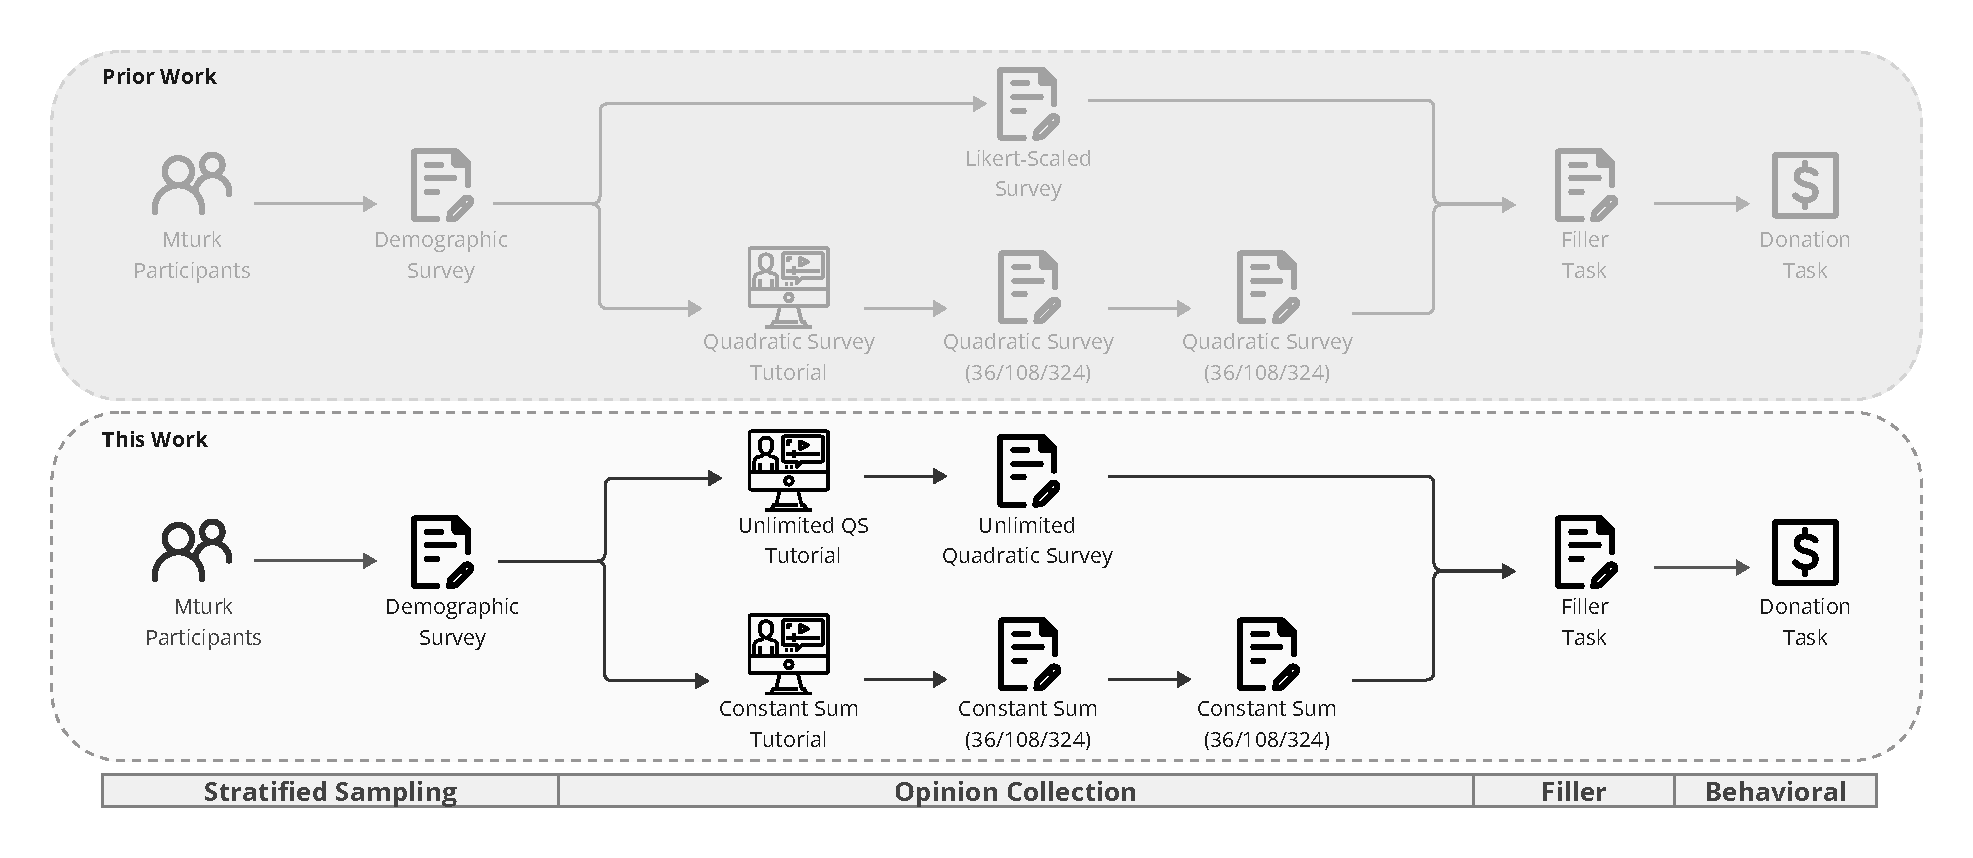
\includegraphics[width=\textwidth]{content/image/whyqs_exp_flow.pdf}
    \caption{Experiment overview. Our study covers the dotted box beneath, mirroring prior research only differing the type of surveys involved during the opinion collection section. The bar below highlights the four parts of the study: sampling, opinion collection, filler task, and the behavioral task.}
    \label{fig:experiment}
\end{figure}

\subsection{Experiment Design}
To ensure comparable data with prior study~\cite{chengCanShowWhat2021}, this study followed the same between-subject experimental design and altered the open sourced software to create two more conditions, creating four new experimental data. Refer to prior studies for details on the procedure justification of the experiment. We highlight key procedures and alternations we made to the methodology below. Figure~\ref{fig:experiment} shows how our study fits into the prior work and the overall experiment flow.

\paragraph{Additional Experimental Conditions}
We added four additional experimental conditions presented as two groups, Unlimited QS or the Constant Sum Survey (CSS) group. The CSS group was further divided into three conditions with different budgets:

\begin{itemize}
    \item **Unlimited QS (UQS):** Participants experience quadratic costs without budget constraints, isolating the effect of cost scaling.
    \item **Constant Sum Survey with 36 Credits (CS36):** A small-budget linear-cost condition testing the effect of budget constraints.
    \item **Constant Sum Survey with 108 Credits (CS108):** A medium-budget version allowing greater expressiveness.
    \item **Constant Sum Survey with 324 Credits (CS324):** A high-budget condition assessing whether increased budgets improve alignment.
\end{itemize}

The UQS condition isolates the effect of quadratic costs, while the CSS conditions isolate the effect of budget constraints. Together, these conditions allow for a direct comparison of cost mechanisms in preference elicitation. As mentioned in~\Cref{sec:related_works_css}, QS with linear cost function is slightly different then CSS where participants do not need to allocate all their provided credits, however, that effectively equals to an additional ``no response'' option on CSS, thus, here we denote these variations as CSS.

Participants assigned to the CSS completed two randomly selected CSS conditions. <report completion time>.

\subsubsection{Survey content}
The study frames the survey as a public resource allotment task, where participants express preferences across 9 societal issues such as education, environment, or health~\footnote{See supplumentary material for the full survey}. Participants would express their degree of preferences in number of votes, positive or negatively under the mechanism of UQS or CSS.

\subsubsection{Surveying process and interface}
Participants in both groups were first introduced to the survey and how to use it via a video tutoiral that we recorded. To assure their understanding of these mechanism, participants were asked to complete a quiz with 5 multiple-choice questions. Participants were required to answer at least 3 questions correctly to continue with the study. We altered the questions based on the survey mechanisms.

The number of credits for the CSS mirros those in the prior study since CSS literature does not provide a clear guideline on how to set the budget with the convension that the budget should be 100. The interface for both studies are shown in~\Cref{fig:extended_interface}.

\subsubsection{Filler task and donation}
After the survey, participants completed a filler task to prevent direct association with the issues and the charities listed on the donation task page. Participants 

\subsubsection{Debrief, and Compensation}
After the study, participants have a chance to read about the study's real purpose on the debrief page. Participants were compensated with \$1.50 for their time, and they were informed that they would receive an additional \$0.50 if they completed the study.

\subsection{Quantitative Measures: Ordinal and Interval Measures}
\label{sec:quantitative_measures}


In the prior studies, the authors used cosine similiarity to measure the alignment between the participants' preferences and their behaviors. However, this measure while useful in tackling high-dimensional data, it risks errors in interpretation. For example, an alignment deemed high by cosine similarity could be due to a large difference in the angle between two vectors with completely aligned rankings compared to a low cosine similarity value that could be due to a small difference in the angle between two vectors with completely unaligned rankings. Based on prior literature in evaluating the effectiveness of CSS, many relied on seperate evaluations of both rankings and intervals between options to evaluate.

In this study, we constructed two Bayesian model to evaluate both ordinal and interval measures of participants' survey results and behaviors.



\subsubsection{Pairwise Ordinal Measures}
\label{sec:ordinal_measures}
The first analysis, which we termed~\textbf{sign analysis}, focuses on understanding how the outcomes from different instruments align with participants' donation behavior in terms of preference order. To achieve this, we construct pairwise comparisons between the two sets. 

After removing participants that made zero donations, for each pairwise option on a survey, we modeled $y_i$ as the outcome variable of whether the order of the two options expressed through the instrument aligns with the order of the donated amount. In other words, our model learns how well does a given survey instrument capture the preference between two options with their donation amount? Since the possible outcome would be either align or misaligned ($\pm 1$), we modeled the outcome variable $y_i$ as a Bernoulli distribution (Equation~\ref{eq:ordinal_model_overall}).

\begin{equation}
    \label{eq:ordinal_model_overall}
    y_i \sim \text{Bernoulli}(\theta_i)
\end{equation}

\begin{equation}
    \label{eq:ordinal_model_logit}
    \text{logit}(\theta_i) = \alpha + \beta_c[C_i] + \beta_o[O_i] + \beta_p[P_i] + \beta_t[T_{1i}] + \beta_t[T_{2i}]
\end{equation}

The model $\theta_i$ is modeled as a logit function (Equation~\ref{eq:ordinal_model_logit}) between pairwise topics $T_{1i}$ and $T_{2i}$, which we control for the specific survey instrument $C_i$. We also control for the order for which participants complete the survey in the QS and LS conditions, denoted as $O_i$ and if so, if the participants was already aligned in a prior condition, $P_i$. The latter two experiment variable help control for potential learning effects since the two survey only differ in the number of provided budgets.

We applied a hiarchical approach to model these experimental variables with a non-centered parameterization~\cite{mcelreath2018statistical}. The hierarchical approach allows partial polling across different pairwise comparisons (e.g., considering how the participants consider the same pair of topics), while preventing overfitting. With so many experimental variables to model under this setup, we applied a non-centered parameterization allows the model to learn the distribution of the parameters from the data rather than being overly constrained by the priors~\cite{mcelreath2018statistical}. This yields more robust inferences, improves sampling efficiency and stability of the model.

This means that for each experimental variable, it follows Equation~\ref{eq:generic_non_center_hyper} where the different possible values of the variable are modeled as a normal distribution with mean $\mu_x$ and standard deviation $\sigma_x$.

\begin{equation}
    \label{eq:generic_non_center_hyper}
    x_i = \mu_x + \sigma_x \cdot \eta_i, \quad \eta_i \sim \mathcal{U}(0,1)
\end{equation}

Each sigma is drawn from a normal distribution with different hyperpriors for each variable. For example, $C_i$ which represents different experiment condition's survey instrument follow the following model:

\begin{align}
    \label{eq:generic_non_center_hyper_C}
    \beta_c[c_i] = \beta_a + \sigma_c \cdot \eta[c_i]\\
    \quad \sigma_c \sim \mathcal{U}(0,1)\\
    \quad \beta_a \sim \mathcal{N}(0, 0.5)\\
    \quad \eta[c_i] \sim \mathcal{N}(0, 1)
\end{align}

The rest of the experimental variables follows the same structure, with the only difference in the hyperprior distribution $\mu_x$. For example, the topics $T_{1i}$ and $T_{2i}$ has a hyperprior of $\mathcal{N}(0, 0.25)$, while the rest of the experimental variables have a hyperprior of $\mathcal{N}(0, 0.5)$. 

\subsubsection{Interval Measures}
\label{sec:interval_measures}
Following the ordinal comparisons,~\textbf{intensity model} assesses how effectively instruments capture the magnitude of preference differences between options. This model evaluates how well an instrument reflects varying degrees of preference along a continuum.

\paragraph{Aligning the variables} Constructing a intensity model to compare the different instruments is not trivial, since elicited values are continuous and others are ordinal. We took a conservative approach and model Likert scale and QS votes as ordinal values, especially when it is not clear whether participants considering the varying costs associated with different votes for the latter. In contrast, LS reflects incremental additions on a scale, and UQS does not have a limit; hence, both are treated as continuous. Rather than solely using final outcomes from each instrument, we also incorporated the cost of votes for QSs, assuming each dollar increment shares the same ``monetary'' value.

For instruments with bounded, continuous budgets (e.g., \textit{QSC\_36}, \textit{QSC\_108}, \textit{QSC\_324}) and linear surveys (\textit{LS\_18}, \textit{LS\_54}, \textit{LS\_162}), we project vote differences onto the $[0,1]$ interval. Since UQS lacks fixed bounds, we normalize the vote difference $V$ between two options $t_1$ and $t_2$ over the $k'$ options that the participant voted on:

\begin{equation}
    \text{Vote\_diff}_{UQS} 
    = (V_{t1} - V_{t2})/\textstyle\sum V_{k'}
\end{equation}
and apply the same normalization for UQS credits.

\paragraph{Projecting Ordinal values} 
To facilitate a direct comparison, we transform the ordinal results into an unobserved latent continuous variable using a Dirichlet-based ``cutpoint'' transformation. Specifically, for each instrument, we derive $K$ discrete ordinal \emph{difference} categories. For example, QS36 has 17 possible difference categories (ranging from $-8$ to $+8$)\footnote{Here, 36 credits can generate a largest difference of 5 votes vs.\ $-3$ votes.}. We then sample
\(\boldsymbol{\alpha}\) from a Dirichlet$(\mathbf{1}\cdot\delta)$ prior, where each of its $K-1$ positive components sums to 1:

\begin{equation}
    \boldsymbol{\alpha} \sim \mathrm{Dirichlet}\bigl(\mathbf{1}\cdot \delta\bigr)
\end{equation}

We modeled the distribution with $\delta=2$ as a weakly informative prior over the latent cutpoints. We pad this vector so that $\alpha_0 = 0$, then map each category $k$ to a latent continuous value:

\begin{equation}
    x_{\mathrm{latent}}^{(k)} = \sum_{j=0}^{k} \alpha_j.
\end{equation}

As $k$ increases, $x_{\mathrm{latent}}^{(k)}$ grows but remains within the $[0,1]$ interval, effectively assigning each ordinal category a continuous value. 

\paragraph{Projecting Donations} Finally, since donation amounts also vary by participant, we remove those who donated nothing and normalize each donation difference by the participant's total donation, mirroring our UQS approach. With these transformations, all experimental variables and outcomes lie in $[0,1]$, forming the basis for a \emph{hierarchical normal} model.

\paragraph{Modeling the outcome}
We seek to capture how an instrument \emph{predicts} the donation difference $y_i$ between two options. Conditional on a mean $\mu_i$, the outcome follows a normal distribution:

\begin{equation}
    \label{eq:intensity_normal}
    y_i \sim \mathcal{N}(\mu_i, \sigma_i).
\end{equation}

where $C_i$ denotes the survey instrument (Likert, QS, QS cost, LS, or UQS). We place a prior $\mathcal{N}(0,0.2)$ on the intercept $\beta_{c}[C_i]$ for each condition and use a non-centered parameterization~\cite{mcelreath2018statistical} to model condition-specific slopes:

\begin{equation}
    \beta_{\text{vote}}[C_i]
    \;=\;
    \beta_{\text{vote}\,\text{bar}}
    + \sigma_{\text{vote}}\,\eta_{\text{vote}}[C_i],
    \quad
    \beta_{\text{vote}\,\text{bar}}
    \sim
    \mathcal{N}(0,1),
    \quad
    \sigma_{\text{vote}}
    \sim
    \mathrm{Uniform}(0,1),
    \quad
    \eta_{\text{vote}}[C_i]
    \sim
    \mathcal{N}(0,1).
\end{equation}

These slopes, together with each instrument's intercept, determine how normalized vote differences $\text{VoteDiff}_i$ (either transformed ordinal or inherently continuous) map onto $y_i$. We also include an order effect $\beta_{o}[O_i]$ and topic intercepts $\beta_{t}[T_{1i}]$ and $\beta_{t}[T_{2i}]$, each following a non-centered prior with a Normal hyper-mean and a Uniform hyper-scale. Putting these elements together, the linear predictor is:

\begin{equation}
    \label{eq:intensity_linpred}
    \mu_i
    =
    \beta_{c}[C_i]
    +
    \beta_{\text{vote}}[C_i] \cdot \text{VoteDiff}_i
    +
    \beta_{o}[O_i]
    +
    \beta_{t}[T_{1i}]
    +
    \beta_{t}[T_{2i}].
\end{equation}

Each condition is then assigned its own standard deviation $\sigma_i=\beta_{\sigma}[C_i]$, where $\beta_{\sigma}[C_i]$ is drawn from an $\mathrm{Exponential}(1)$ prior. Hence, different instruments exhibit distinct variance in donation differences.

A hierarchical Bayesian approach ties all these parameters together via a non-centered parameterization:

\begin{equation}
    x_i
    =
    \mu_x
    + \sigma_x \cdot \eta_i,
    \qquad
    \eta_i
    \sim
    \mathcal{N}(0,1).
\end{equation}

Here, $\mu_x$ and $\sigma_x$ define the group-level mean and scale for each parameter type, and $x_i$ represents condition intercepts, slopes, order intercepts, or topic intercepts. By integrating condition, vote difference, order, and topic effects into a single hierarchical normal framework, our model provides a structured way to analyze how different survey instruments capture the intensity of preference differences.

